\subsection{Local environment and structural response}

We next examine the local metal coordination around the Pt adsorption sites,
the relation between the binding energy and the \ce{Pt-C} distance, and the
changes in the \ce{C-O} bond length and stretching frequency.
The ECoN procedure and notation are defined in the Methods section. The
pre-adsorption descriptors for the derivative structures are collected
in Table~\ref{tab:tfg_crossed_ptge_econ_descriptors}; using the bare-cluster
geometry separates the initial site environment from the structural response
induced by adsorption. The corresponding descriptors for the GM structures
are reported in Supporting Table~\ref{tab:tfg_gm_ptge_econ_pre_descriptors}.

For \ce{Pt6Ge4^{der}}, site 5/7 has the largest initial Ge fraction
($x_{\rm Ge}^{0}=0.809$) and gives the weakest CO binding in the series
($BE_{\rm ad}(\ce{CO})=-1.57$ eV). By contrast, sites 2 and 1/4 combine substantial effective
Pt coordination with smaller $x_{\rm Ge}^{0}$ values and give three of the
strongest binding energies. This comparison is consistent with weaker CO
binding as the Ge contribution to the initial Pt environment increases.
{Site 9 is an exception. Although its initial Ge fraction is relatively
large ($x_{\rm Ge}^{0}=0.751$), its binding energy ($-2.25$ eV) is nearly the same as}
those of sites 2 and 1/4. Upon adsorption, however, the local environment of
site 9 changes appreciably: $ECoN_{\rm Pt}^{0}=0.727$ increases to
$ECoN_{\rm Pt}^{\ce{CO}}=1.163$, while $x_{\rm Ge}^{0}=0.751$ decreases to
$x_{\rm Ge}^{\ce{CO}}=0.614$. The corresponding changes at site 5/7 are
smaller: $ECoN_{\rm Pt}$ increases from 0.529 to 0.657 and $x_{\rm Ge}$
decreases from 0.809 to 0.771. Thus, the optimized site-9 carbonyl has a larger
effective Pt contribution than its initial environment suggests. This local
{reorganization may help explain why site 9 departs from the initial
trend. However, these ECoN changes describe the final local environment and
do not quantify the energetic contribution of reorganization.} The initial
local composition therefore contributes to the observed pattern but does not
determine the binding energy by itself. The descriptors of the optimized
carbonyls are reported in Supporting
Table~\ref{tab:tfg_crossed_ptge_econ_co_descriptors}.

The $ECoN_{\rm Pt}^{0}$ and $ECoN_{\rm Ge}^{0}$ components, which measure the
effective contributions from neighboring Pt and Ge atoms, respectively,
provide complementary information for \ce{Pt5Ge5^{der}}.
Site 4, which gives the weakest adsorption in this composition, has
$x_{\rm Ge}^{0}\simeq1$ and essentially no effective Pt coordination. By
contrast, sites 6/8 and 7/10 have almost identical $x_{\rm Ge}^{0}$ values,
but their total effective coordination numbers differ markedly (about 5.58
and 2.91, respectively), together with a 0.42~eV difference in binding energy.
This difference in total coordination is largely retained after adsorption:
$ECoN_{\rm total}^{\ce{CO}}$ is 5.69 for site 6/8 and 2.95 for site 7/10,
increases of only 0.11 and 0.05, respectively. In both carbonyls,
$x_{\rm Ge}$ decreases ($0.745$ to $0.703$ for site 6/8 and $0.746$ to
$0.683$ for site 7/10), indicating a shift in the local coordination balance
toward Pt. Thus, the two sites retain very different total coordination after
CO adsorption despite having similar Ge fractions. This comparison describes
how their local environments change, but does not by itself explain the
0.42~eV difference in binding energy.

For \ce{Pt4Ge6^{der}}, all sampled sites are Ge-rich, but the pre-adsorption
descriptors clarify the weakest-binding structure. Site 1 has
$x_{\rm Ge}^{0}=0.980$ and $ECoN_{\rm Pt}^{0}=0.089$, showing that the
adsorbing Pt atom is initially almost completely coordinated by Ge. Sites 5
and 7 have different initial ECoN descriptors and are therefore listed
separately in Table~\ref{tab:tfg_crossed_ptge_econ_descriptors}, although both
adsorption trajectories converge to the same carbonyl minimum and give the
same binding energy. Together with site 2, they retain larger effective
contributions from Pt than site 1 and bind CO more strongly. Upon adsorption,
however, site 1 undergoes substantial local
reorganization: $ECoN_{\rm Pt}^{\ce{CO}}$ increases to 1.423 and
$x_{\rm Ge}^{\ce{CO}}$ falls to 0.759. The ECoN descriptors of the optimized
derivative carbonyls are reported in Supporting
Table~\ref{tab:tfg_crossed_ptge_econ_co_descriptors}, while the corresponding
final-state descriptors for the GM structures are given in Supporting
Table~\ref{tab:tfg_gm_ptge_econ_descriptors}.

We next use the GM series to examine whether the relation between the
initial Pt/Ge environment and CO binding found above persists when the starting
cluster isomer is changed. For \ce{Pt6Ge4^{GM}}, the four sites with
$x_{\rm Ge}^{0}=0.337$--0.563 give the strongest triplet binding energies
($-1.95$ to $-1.66$~eV), whereas sites 4 and 5 have more Ge-rich initial
environments ($x_{\rm Ge}^{0}=0.807$ and 0.802) and give the weakest values
($-1.21$ and $-1.22$~eV). A similar distinction is found for \ce{Pt5Ge5^{GM}}:
sites 1, 2, 4, and 5
have $x_{\rm Ge}^{0}=0.929$--0.930 and converge to the same carbonyl minimum,
whereas site 3 is almost completely coordinated by Ge
($x_{\rm Ge}^{0}=0.998$) and gives the weakest binding. The \ce{Pt4Ge6^{GM}}
series is less regular. All four sites are Ge-rich. Sites 2 and 3 have similar
initial Ge fractions (0.920 and 0.905), yet they give the strongest and weakest
binding energies, respectively ($-1.51$ and $-1.05$ eV). {Thus, the
initial ECoN descriptors distinguish important features of the adsorption
environment, but they do not determine the full binding-energy order.}

{Overall, the initial ECoN descriptors show that Pt sites with a larger
Ge contribution generally bind \ce{CO} less strongly.}
{The exception at site 9 of \ce{Pt6Ge4^{der}} and the variation across the
\ce{Pt4Ge6^{GM}} series show that ECoN describes the initial local
environment, but does not by itself determine the binding-energy order. We next examine the optimized Pt–C and C–O bond lengths and the CO stretching frequency to characterize the carbonyl after relaxation.}

\begin{table}[H]
\begin{center}
\caption{Local Hoppe ECoN descriptors for each Pt adsorption site in the bare
\ce{Pt10}-to-\ce{Pt-Ge} clusters, before \ce{CO} is added. The superscript 0
denotes this pre-adsorption geometry. Only metal neighbors are included, and
$ECoN_{\rm total}^{0}=ECoN_{\rm Pt}^{0}+ECoN_{\rm Ge}^{0}$ and
$x_{\rm Ge}^{0}=ECoN_{\rm Ge}^{0}/ECoN_{\rm total}^{0}$. Paired labels denote
initial positions represented by the same listed descriptors and adsorption
result. Sites 5 and 7 of \ce{Pt4Ge6CO} are listed separately because their
initial ECoN descriptors differ, although they converge to the same carbonyl
minimum.}
\label{tab:tfg_crossed_ptge_econ_descriptors}
\small
\begin{tabular}{lcrrrrr}
\toprule
{System} &  {Site} & {$BE_{\rm ad}(\ce{CO})$ / eV} &
{$ECoN_{\rm total}^{0}$} & {$ECoN_{\rm Pt}^{0}$} & {$ECoN_{\rm Ge}^{0}$} &
{$x_{\rm Ge}^{0}$} \\
\midrule
\ce{Pt6Ge4^{der}CO}  & 2  & -2.25 & 3.22 & 1.88 & 1.34 & 0.42 \\
\ce{Pt6Ge4^{der}CO}  & 9  & -2.25 & 2.92 & 0.73 & 2.19 & 0.75 \\
\ce{Pt6Ge4^{der}CO}  & 1/4  & -2.24 & 4.60 & 2.70 & 1.90 & 0.41 \\
\ce{Pt6Ge4^{der}CO}  & 5/7  & -1.57 & 2.77 & 0.53 & 2.24 & 0.81 \\
\midrule
\ce{Pt5Ge5^{der}CO}  & 6/8  & -2.08 & 5.58 & 1.42 & 4.16 & 0.75 \\
\ce{Pt5Ge5^{der}CO}  & 7/10 & -1.66 & 2.91 & 0.74 & 2.17 & 0.75 \\
\ce{Pt5Ge5^{der}CO}  & 4  & -1.34 & 2.95 & 0.00 & 2.95 & 1.00 \\
\midrule
\ce{Pt4Ge6^{der}CO}  & 5  & -1.46 & 3.99 & 0.56 & 3.43 & 0.86 \\
\ce{Pt4Ge6^{der}CO}  & 7  & -1.46 & 3.48 & 0.28 & 3.20 & 0.92 \\
\ce{Pt4Ge6^{der}CO}  & 2  & -1.31 & 4.71 & 0.47 & 4.25 & 0.90 \\
\ce{Pt4Ge6^{der}CO}  & 1  & -1.05 & 4.41 & 0.09 & 4.32 & 0.98 \\
\bottomrule
\end{tabular}
\end{center}
\end{table}

\begin{figure}[H]
\centering
\definecolor{ptten}{RGB}{0,0,0}
\definecolor{ptsixgefour}{RGB}{0,114,178}
\definecolor{ptfivegefive}{RGB}{213,94,0}
\definecolor{ptfourgesix}{RGB}{0,158,115}

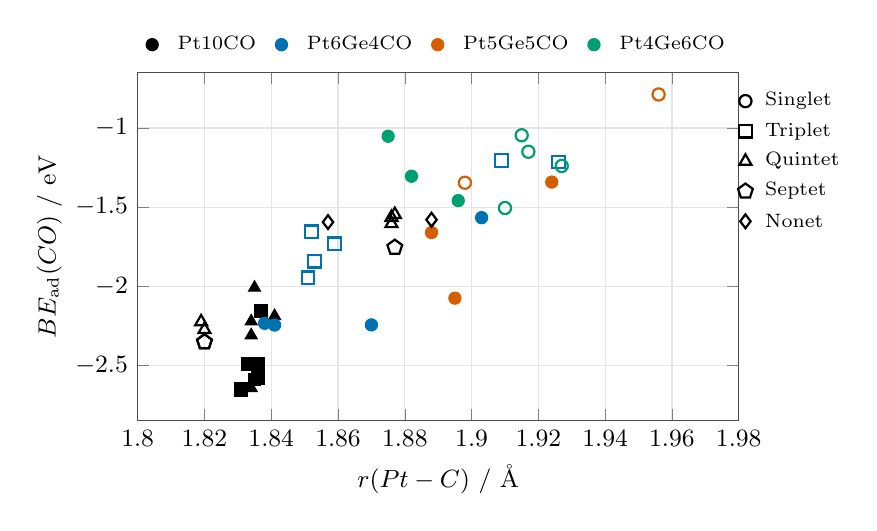
\begin{tikzpicture}
\begin{axis}[
  width=0.76\linewidth,
  height=6.0cm,
  xmin=1.80, xmax=1.98,
  ymin=-2.85, ymax=-0.65,
  xlabel={$r(\ce{Pt-C})$ / \AA},
  ylabel={$BE_{\rm ad}(\ce{CO})$ / eV},
  ylabel style={yshift=-2pt},
  tick label style={font=\small},
  label style={font=\small},
  grid=major,
  grid style={gray!20},
  axis line style={black!70},
  clip=false,
  legend style={at={(0.5,1.03)},anchor=south,draw=none,inner sep=1pt,
    font=\scriptsize,legend columns=4,column sep=5pt}
]
\addlegendimage{only marks,mark=*,mark size=2.2pt,ptten}
\addlegendentry{\ce{Pt10CO}}
\addlegendimage{only marks,mark=*,mark size=2.2pt,ptsixgefour}
\addlegendentry{\ce{Pt6Ge4CO}}
\addlegendimage{only marks,mark=*,mark size=2.2pt,ptfivegefive}
\addlegendentry{\ce{Pt5Ge5CO}}
\addlegendimage{only marks,mark=*,mark size=2.2pt,ptfourgesix}
\addlegendentry{\ce{Pt4Ge6CO}}
% Filled symbols: atom-substitution models.
\addplot[only marks,mark=square*,mark size=2.3pt,ptten] coordinates {
  (1.831,-2.657) (1.831,-2.650) (1.835,-2.590) (1.836,-2.579)
  (1.833,-2.493) (1.836,-2.493) (1.837,-2.156)};
\addplot[only marks,mark=triangle*,mark size=2.5pt,ptten] coordinates {
  (1.834,-2.645) (1.834,-2.311) (1.834,-2.223) (1.841,-2.189)
  (1.835,-2.010)};
\addplot[only marks,mark=*,mark size=2.2pt,ptsixgefour] coordinates {
  (1.841,-2.246) (1.870,-2.245) (1.838,-2.235) (1.903,-1.567)};
\addplot[only marks,mark=*,mark size=2.2pt,ptfivegefive] coordinates {
  (1.895,-2.076) (1.888,-1.661) (1.924,-1.342)};
\addplot[only marks,mark=*,mark size=2.2pt,ptfourgesix] coordinates {
  (1.896,-1.459) (1.882,-1.305) (1.875,-1.052)};
% Open symbols: models initiated from the global-minimum parent.
\addplot[only marks,mark=triangle,mark size=2.5pt,ptten,
  mark options={fill=white,draw=ptten,line width=0.8pt}] coordinates {
  (1.820,-2.275) (1.819,-2.226) (1.876,-1.605) (1.876,-1.566)
  (1.877,-1.547)};
\addplot[only marks,mark=pentagon,mark size=2.8pt,ptten,
  mark options={fill=white,draw=ptten,line width=0.8pt}] coordinates {
  (1.820,-2.353) (1.820,-2.353) (1.877,-1.755)};
\addplot[only marks,mark=diamond,mark size=2.5pt,ptten,
  mark options={fill=white,draw=ptten,line width=0.8pt}] coordinates {
  (1.857,-1.595) (1.888,-1.580)};
\addplot[only marks,mark=square,mark size=2.3pt,ptsixgefour,
  mark options={fill=white,draw=ptsixgefour,line width=0.8pt}] coordinates {
  (1.851,-1.947) (1.853,-1.842) (1.859,-1.732) (1.852,-1.657)
  (1.926,-1.215) (1.909,-1.207)};
\addplot[only marks,mark=o,mark size=2.2pt,ptfivegefive,
  mark options={fill=white,draw=ptfivegefive,line width=0.8pt}] coordinates {
  (1.898,-1.346) (1.956,-0.788)};
\addplot[only marks,mark=o,mark size=2.2pt,ptfourgesix,
  mark options={fill=white,draw=ptfourgesix,line width=0.8pt}] coordinates {
  (1.910,-1.506) (1.927,-1.240) (1.917,-1.150) (1.915,-1.046)};
% Symbol key: fill is reserved for the structural-parent distinction.
\addplot[only marks,mark=o,mark size=2.2pt,black,
  mark options={fill=white,draw=black,line width=0.8pt}] coordinates {(1.982,-0.83)};
\node[anchor=west,font=\scriptsize] at (axis cs:1.985,-0.83) {Singlet};
\addplot[only marks,mark=square,mark size=2.3pt,black,
  mark options={fill=white,draw=black,line width=0.8pt}] coordinates {(1.982,-1.02)};
\node[anchor=west,font=\scriptsize] at (axis cs:1.985,-1.02) {Triplet};
\addplot[only marks,mark=triangle,mark size=2.5pt,black,
  mark options={fill=white,draw=black,line width=0.8pt}] coordinates {(1.982,-1.21)};
\node[anchor=west,font=\scriptsize] at (axis cs:1.985,-1.21) {Quintet};
\addplot[only marks,mark=pentagon,mark size=2.8pt,black,
  mark options={fill=white,draw=black,line width=0.8pt}] coordinates {(1.982,-1.40)};
\node[anchor=west,font=\scriptsize] at (axis cs:1.985,-1.40) {Septet};
\addplot[only marks,mark=diamond,mark size=2.5pt,black,
  mark options={fill=white,draw=black,line width=0.8pt}] coordinates {(1.982,-1.59)};
\node[anchor=west,font=\scriptsize] at (axis cs:1.985,-1.59) {Nonet};
\end{axis}
\end{tikzpicture}

\caption{Binding energy versus the optimized \ce{Pt-C} distance for the
carbonyls. Black, blue, vermilion, and green identify \ce{Pt10CO},
\ce{Pt6Ge4CO}, \ce{Pt5Ge5CO}, and \ce{Pt4Ge6CO}, respectively. Filled symbols
denote derivative structures and open symbols denote structures initiated
from the corresponding global-minimum structure. Circles, squares, triangles,
pentagons, and diamonds represent singlet, triplet, quintet, septet, and
nonet states, respectively.}
\label{fig:neutral_be_vs_ptc}
\end{figure}

\begin{figure}[H]
\centering
\definecolor{ptten}{RGB}{0,0,0}
\definecolor{ptsixgefour}{RGB}{0,114,178}
\definecolor{ptfivegefive}{RGB}{213,94,0}
\definecolor{ptfourgesix}{RGB}{0,158,115}

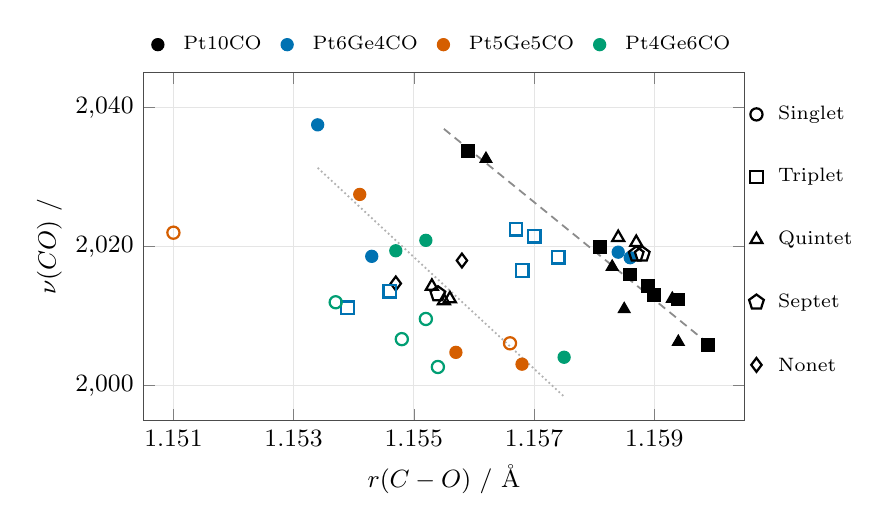
\begin{tikzpicture}
\begin{axis}[
  width=0.76\linewidth,
  height=6.0cm,
  xmin=1.1505, xmax=1.1605,
  ymin=1995, ymax=2045,
  xlabel={$r(\ce{C-O})$ / \AA},
  ylabel={$\nu(\ce{CO})$ / \si{\per\centi\metre}},
  ylabel style={yshift=-2pt},
  xtick={1.151,1.153,1.155,1.157,1.159},
  xticklabel style={/pgf/number format/fixed,/pgf/number format/precision=3},
  ytick={2000,2020,2040},
  tick label style={font=\small},
  label style={font=\small},
  grid=major,
  grid style={gray!20},
  axis line style={black!70},
  clip=false,
  legend style={at={(0.5,1.03)},anchor=south,draw=none,inner sep=1pt,
    font=\scriptsize,legend columns=4,column sep=5pt}
]
\addlegendimage{only marks,mark=*,mark size=2.2pt,ptten}
\addlegendentry{\ce{Pt10CO}}
\addlegendimage{only marks,mark=*,mark size=2.2pt,ptsixgefour}
\addlegendentry{\ce{Pt6Ge4CO}}
\addlegendimage{only marks,mark=*,mark size=2.2pt,ptfivegefive}
\addlegendentry{\ce{Pt5Ge5CO}}
\addlegendimage{only marks,mark=*,mark size=2.2pt,ptfourgesix}
\addlegendentry{\ce{Pt4Ge6CO}}
% Visual guides for the filled atom-substitution data sets only; no regression is implied.
\addplot[black!45,densely dashed,line width=0.65pt]
  coordinates {(1.15550,2036.92) (1.16000,2005.35)};
\addplot[gray!60,densely dotted,line width=0.65pt]
  coordinates {(1.15340,2031.32) (1.15750,1998.44)};
% Filled symbols: atom-substitution models.
\addplot[only marks,mark=square*,mark size=2.3pt,ptten] coordinates {
 (1.1581,2020.0) (1.1594,2012.4) (1.1589,2014.3) (1.1590,2013.0)
 (1.1599,2005.9) (1.1586,2016.0) (1.1559,2033.7)};
\addplot[only marks,mark=triangle*,mark size=2.5pt,ptten] coordinates {
 (1.1593,2012.5) (1.1583,2017.1) (1.1562,2032.6) (1.1585,2011.0)
 (1.1594,2006.3)};
\addplot[only marks,mark=*,mark size=2.2pt,ptsixgefour] coordinates {
 (1.1584,2019.2) (1.1534,2037.5) (1.1586,2018.4) (1.1543,2018.6)};
\addplot[only marks,mark=*,mark size=2.2pt,ptfivegefive] coordinates {
 (1.1568,2003.1) (1.1541,2027.5) (1.1557,2004.8)};
\addplot[only marks,mark=*,mark size=2.2pt,ptfourgesix] coordinates {
 (1.1547,2019.4) (1.1552,2020.9) (1.1575,2004.1)};
% Open symbols: models initiated from the global-minimum parent.
\addplot[only marks,mark=triangle,mark size=2.5pt,ptten,
  mark options={fill=white,draw=ptten,line width=0.8pt}] coordinates {
 (1.1584,2021.3) (1.1587,2020.6) (1.1553,2014.3) (1.1556,2012.5)
 (1.1555,2012.2)};
\addplot[only marks,mark=pentagon,mark size=2.8pt,ptten,
  mark options={fill=white,draw=ptten,line width=0.8pt}] coordinates {
 (1.1587,2018.9) (1.1588,2018.9) (1.1554,2013.2)};
\addplot[only marks,mark=diamond,mark size=2.5pt,ptten,
  mark options={fill=white,draw=ptten,line width=0.8pt}] coordinates {
 (1.1558,2018.0) (1.1547,2014.7)};
\addplot[only marks,mark=square,mark size=2.3pt,ptsixgefour,
  mark options={fill=white,draw=ptsixgefour,line width=0.8pt}] coordinates {
 (1.1574,2018.5) (1.1567,2022.5) (1.1568,2016.6) (1.1570,2021.5)
 (1.1539,2011.2) (1.1546,2013.6)};
\addplot[only marks,mark=o,mark size=2.2pt,ptfivegefive,
  mark options={fill=white,draw=ptfivegefive,line width=0.8pt}] coordinates {
 (1.1566,2006.1) (1.1510,2022.0)};
\addplot[only marks,mark=o,mark size=2.2pt,ptfourgesix,
  mark options={fill=white,draw=ptfourgesix,line width=0.8pt}] coordinates {
 (1.1552,2009.6) (1.1537,2012.0) (1.1548,2006.7) (1.1554,2002.7)};
% Symbol key: fill is reserved for the structural-parent distinction.
\addplot[only marks,mark=o,mark size=2.2pt,black,
  mark options={fill=white,draw=black,line width=0.8pt}] coordinates {(1.1607,2039)};
\node[anchor=west,font=\scriptsize] at (axis cs:1.1609,2039) {Singlet};
\addplot[only marks,mark=square,mark size=2.3pt,black,
  mark options={fill=white,draw=black,line width=0.8pt}] coordinates {(1.1607,2030)};
\node[anchor=west,font=\scriptsize] at (axis cs:1.1609,2030) {Triplet};
\addplot[only marks,mark=triangle,mark size=2.5pt,black,
  mark options={fill=white,draw=black,line width=0.8pt}] coordinates {(1.1607,2021)};
\node[anchor=west,font=\scriptsize] at (axis cs:1.1609,2021) {Quintet};
\addplot[only marks,mark=pentagon,mark size=2.8pt,black,
  mark options={fill=white,draw=black,line width=0.8pt}] coordinates {(1.1607,2012)};
\node[anchor=west,font=\scriptsize] at (axis cs:1.1609,2012) {Septet};
\addplot[only marks,mark=diamond,mark size=2.5pt,black,
  mark options={fill=white,draw=black,line width=0.8pt}] coordinates {(1.1607,2003)};
\node[anchor=west,font=\scriptsize] at (axis cs:1.1609,2003) {Nonet};
\end{axis}
\end{tikzpicture}

\caption{Harmonic \ce{C-O} stretching frequency versus the optimized
\ce{C-O} distance for the carbonyls. Black, blue, vermilion, and green identify
\ce{Pt10CO}, \ce{Pt6Ge4CO}, \ce{Pt5Ge5CO}, and \ce{Pt4Ge6CO}, respectively.
Filled symbols denote derivative structures and open symbols denote
structures initiated from the corresponding global-minimum structure. Circles,
squares, triangles, pentagons, and diamonds represent singlet, triplet,
quintet, septet, and nonet states, respectively. The dashed black line is a
visual guide through the filled \ce{Pt10CO} triplet and quintet points. The
dotted gray line is a visual guide through the region occupied by most filled
Pt--Ge singlet points; it is not a regression line. The two filled
\ce{Pt6Ge4CO} structures initiated at site class 1/4 and site 2 fall clearly outside this
region.}
\label{fig:neutral_co_frequency}
\end{figure}

Figure~\ref{fig:neutral_be_vs_ptc} shows a broad trend, where shorter optimized
\ce{Pt-C} contacts generally correspond to more negative \ce{CO} binding
energies. The scatter, however, shows that the Pt--C distance alone does not
determine the adsorption energy.

For the \ce{Pt10^{der}CO}
series, the triplet minima have very similar \ce{Pt-C} distances,
1.83--1.84~\si{\angstromunit}, although their binding energies span about 0.50 eV (black
filled squares in
Figure~\ref{fig:neutral_be_vs_ptc}). The
\blue{Quintet minima (black filled triangles) show the same pattern. Their distances
cover only 1.83--1.84~\si{\angstromunit}, whereas their binding energies span
about 0.64 eV.} The GM data (open symbols) extend the
range of \ce{Pt-C} distances, but they also involve different starting geometries
and spin states. Their broader scatter therefore reflects changes in more than
the \ce{Pt-C} distance alone.

The Pt--Ge carbonyls extend the sampled \ce{Pt-C} range to about
1.96~\si{\angstromunit}. Longer Pt--C contacts are often associated with weaker adsorption,
but this is not a strict relation for all structures. For example, the
\ce{Pt4Ge6CO} derivative structures with similar \ce{Pt-C} distances have
binding energies that differ by several tenths of an eV. The local Pt/Ge
environment and relaxation of the whole cluster must therefore be considered
together with the Pt--C distance.

The internal \ce{C-O} bond connects this larger-cluster analysis with the
Blyholder interpretation used in earlier DFT studies.\cite{ugartemendia:2021,ugartemendia:2022}
The optimized \ce{C-O} distances for the derivative carbonyls are
listed in Supporting Tables~\ref{tab:tfg_adsorption_descriptors} and
\ref{tab:tfg_bimetallic_adsorption_descriptors}. They show a small overall
decrease in \ce{C-O} activation for the Ge-containing clusters, although the
individual structures are not strictly monotonic. This complementary
structural indicator agrees with the previous DFT-based
NBO\cite{ugartemendia:2021} and PDOS\cite{ugartemendia:2022} analyses, and
is consistent with reduced metal-to-\ce{CO} back-donation upon Ge
substitution.

Figure~\ref{fig:neutral_co_frequency} shows the relation between the \ce{C-O}
bond length and stretching frequency for the derivative and GM
carbonyls. Badger's rule
relates the equilibrium bond length to the stretching force constant for the
same atomic pair.\cite{badger:1934,dabo:2012} The filled derivative
\ce{Pt10CO} points show the expected inverse length--frequency pattern. Many
of the filled Pt--Ge singlet points occupy a second, distinct region of the
plot. The dashed black and dotted gray segments are included only as visual
guides to these two regions and are not regression lines. Two derivative
\ce{Pt6Ge4CO} structures, initiated at site class 1/4 and site 2, lie clearly
outside the second region. They have the two longest \ce{C-O} bonds in this
subset (1.16 and 1.16~\si{\angstromunit}), but relatively low stretching
frequencies (2018.4 and 2019.2~\si{\per\centi\metre}). In their optimized structures, the
CO-binding Pt atom has one close Ge neighbor and two close Pt neighbors. This
more Pt-rich local environment is consistent with their stronger adsorption
and greater C--O activation. The global-minimum points are distributed
over a wider part of the plot, both between and outside the two derivative
regions. This broader distribution is observed for several compositions and
for the different \ce{Pt10} spin states, {showing that the distribution
also depends on the starting structure and spin state.}

Overall, the local descriptors give a consistent but incomplete picture.
Shorter \ce{Pt-C} distances and larger \ce{C-O} elongations generally accompany
stronger adsorption, and Ge-rich Pt environments tend to bind \ce{CO} more
weakly. The remaining scatter shows that these quantities must be read together
with the relaxation of the whole cluster, which is examined explicitly below.

